\section*{Informações}

\begin{wrapfigure}{r}{-0.10\textwidth} 
	\centering
	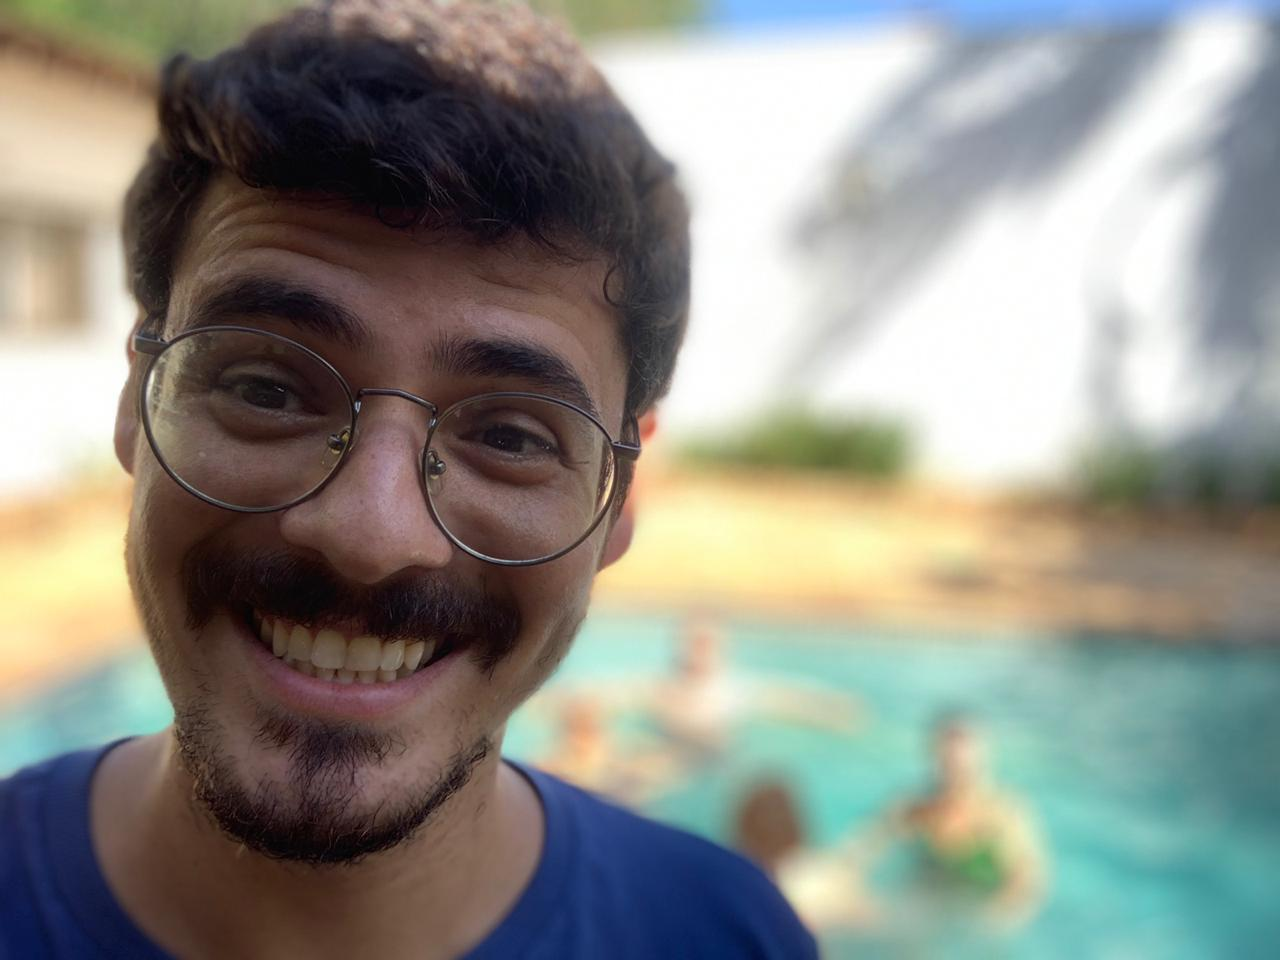
\includegraphics[width=0.35\textwidth]{foto}
\end{wrapfigure}

{\Large \faUser} \textbf{Vanderlei C. Oliveira Jr.}\\
{\Large \faInstitution} \href{https://www.on.br/index.php/pt-br/}{Observatório Nacional}\\
{\Large \faEnvelope} \href{mailto:vanderlei@on.br}{vanderlei@on.br}\\
{\Large \faEnvelopeO} \href{mailto:vandscoelho@gmail.com}{vandscoelho@gmail.com}\\
{\Large \faGroup} \href{http://www.pinga-lab.org/people/oliveira-jr.html}{pinga-lab.org/people/oliveira-jr}\\
{\Large \faInfoCircle} \href{http://lattes.cnpq.br/4332841435949533}{lattes.cnpq.br/4332841435949533}\\
{\Large \faInfoCircle} \href{http://orcid.org/0000-0002-6338-4086}{orcid.org/0000-0002-6338-4086}\\


%%% Education
%%% ------------------------------------------------------------
\section*{Formação}

\subsection*{Doutorado em Geof{\'i}sica}

%\faGraduationCap \quad \textbf{Doutorado em Geof{\'i}sica}\\
\faHourglassStart \quad Dez/2010 -- Jan/2013\\
\faInstitution \quad \href{http://www.on.br/index.php/pt-br/}{Observat{\'o}rio Nacional}\\
\faExternalLink \quad  \href{http://www.pinga-lab.org/thesis/oliveira-jr-phd.html}{Processamento e invers\~{a}o de dados de campos potenciais: Novas abordagens}\\
\textbf{Orientadora:} Dra. Valéria C. F. Barbosa \\
\textbf{Descrição:} Desenvolvi duas metodologias para o 
processamento e interpretação de dados gravimétricos e magnetométricos. A primeira é
a \textit{Camada Equivalente Polinomial} (\textit{Polynomial Equivalent Layer}), que 
é uma metodologia computacionalmente eficiente para processar grandes volumes de dados 
via técnica da camada equivalente. A segunda é uma metodologia para estimar a geometria 
de corpos 3D isolados via inversão não-linear de dados de gradiometria da gravidade.\\


\subsection*{Mestrado em Geof{\'i}sica}

%\faGraduationCap \quad \textbf{Mestrado em Geof{\'i}sica}\\
\faHourglassStart \quad Mar/2009 -- Nov/2010\\
\faInstitution \quad \href{http://www.on.br/index.php/pt-br/}{Observat{\'o}rio Nacional}\\
\faExternalLink \quad  \href{http://www.pinga-lab.org/thesis/oliveira-jr-msc.html}{Invers{\~a}o gravim{\'e}trica radial por camadas para a reconstru{\c c}{\~a}o de corpos geol{\'o}gicos 3D}\\
\textbf{Orientadora:} Dra. Valéria C. F. Barbosa \\
\textbf{Descrição:} Desenvolvi uma metodologia para
estimar a geometria de um corpo geol{\'o}gico 3D via invers{\~a}o n{\~a}o-linear 
de dados gravimétricos.\\


\subsection*{Bacharelado em Geof{\'i}sica}

%\faGraduationCap \quad \textbf{Bacharelado em Geof{\'i}sica}\\
\faHourglassStart \quad Mar/2004 -- Dez/2008\\
\faInstitution \quad \href{https://www.iag.usp.br/}{Instituto de Astronomia, Geof{\'i}sica e Ci{\^e}ncias Atmosf{\'e}ricas da Universidade de S{\~a}o Paulo}\\
\faExternalLink \quad Modelagem gravim{\'e}trica 3D da borda norte da Bacia do Paran{\'a}\\
\textbf{Orientadora:} Dra. Yára R. Marangoni \\
\textbf{Descrição:} Apliquei uma metodologia para estimar a geometria do 
embasamento e da Moho a partir da inversão não-linear de dados gravimétricos 
sobre a borda norte da Bacia do Paraná.


%\NewPart{Research interests}{}
%
%{\begin{itemize}
%
%	\item{\textbf{Equivalent layer technique:} computationally efficient methods 
%	for processing and interpreting large potential field data sets.}
%	
%	\item{\textbf{Inversion of gravity and/or magnetic data:} methods to invert gravity 
%	and/or magnetic data for the purpose of estimating the position and shape of geological
%	bodies.}
%	
%	\item{\textbf{Magnetization of geological bodies:} methods for estimating the
%	magnetization direction of geological bodies by using land and airborne magnetic data.}
%	
%	\item{\textbf{Magnetization of rock samples:} methods for estimating the magnetization
%	distribution within rock samples by using scanning magnetic microscopy data.}
%	
%	\item{\textbf{Magnetic modeling of geological bodies:} methods for computing the
%	demagnetizing field within geological bodies having high susceptibility.}
%	
%	\item{\textbf{Regional characterization of gravity field:} computationally efficient
%	methods for representing the regional gravity field by combining different data sets.}
%	
%	\item{\textbf{Regional characterization of the crustal magnetic field:} computationally
%	efficient methods for representing the crustal field by combining different data sets.}
%
%\end{itemize}}

%\vspace{2cm}